% SPDX-License-Identifier: CC-BY-4.0
% Copyright (c) 2026 Alexander Stephen Donahue (Independent Researcher, ORCID 0009-0006-8168-9648)
\documentclass[11pt,letterpaper]{amsart}

\usepackage[margin=0.92in]{geometry}
\usepackage{amsmath,amssymb,amsthm}
\usepackage{graphicx}
\usepackage{booktabs}
\usepackage{array}
\usepackage{tabularx}
\usepackage{xcolor}
\usepackage{xurl}
\usepackage{hyperref}
\usepackage{microtype}
\emergencystretch=3em
\raggedbottom
\newcolumntype{L}{>{\raggedright\arraybackslash}X}

\hypersetup{
  colorlinks=true,
  linkcolor=blue!65!black,
  citecolor=blue!65!black,
  urlcolor=blue!65!black,
  pdftitle={An 11-Discipline Open Hard Problems Map from Nanoscale Synaptic Biophysics to the Consciousness Frontier},
  pdfauthor={Alexander Stephen Donahue}
}

\newtheorem{theorem}{Theorem}[section]
\newtheorem{remark}[theorem]{Remark}

\title[11-Discipline Open Problems, Mega-Atlas \& Consciousness Epistemology]{An 11-Discipline Open Hard Problems Map from Nanoscale Synaptic Biophysics to the Consciousness Frontier: Formal Bounds, Mega-Atlas Crosswalk, Deductive--Inductive--Abductive Epistemology, and a Ten-Class Audit}

\author{Alexander Stephen Donahue}
\address{Independent Researcher, Spokane, WA, USA}
\email{0\_0@0thernes.art}
\thanks{ORCID: \href{https://orcid.org/0009-0006-8168-9648}{0009-0006-8168-9648}. Zenodo Concept DOI: \href{https://doi.org/10.5281/zenodo.24477927}{10.5281/zenodo.24477927} (all versions; prior v1.3.0 Version DOI \href{https://doi.org/10.5281/zenodo.24548051}{10.5281/zenodo.24548051}). Companion survey and epistemic-boundary white paper to \texttt{human-synapse-bouton-lab} v1.4.0 (\url{https://github.com/0thernes/human-synapse-bouton-lab}). Interactive Lean Blueprint: \url{https://0thernes.github.io/human-synapse-bouton-lab/blueprint/}. Dual-licensed: Apache-2.0 (code/Lean) and CC-BY-4.0 (manuscript/figures). Preprint; not externally peer-reviewed.}
\date{November 26, 2026}

\begin{document}

\begin{abstract}
Bridging nanoscale synaptic biophysics to human cognition and phenomenal consciousness requires navigating eleven interdependent scientific disciplines---Mathematics, Physics, Chemistry, Biology, Neuroscience, Neuropsychology, NeuroCS, NeuroMath, Neurochemistry, Neurobiology, and Neurophysics---without collapsing into unfalsifiable speculation. This companion survey and epistemic-boundary monograph accompanies \texttt{human-synapse-bouton-lab} v1.4.0; it presents no new standalone formal proof or empirical result beyond the companion technical paper, and instead maps our verified software artifacts cleanly against open scientific problems. We stratify every claim across four strict epistemic tiers: (1)~\emph{kernel-checked elementary algebraic and discrete-dynamical lemmas} verified in Lean~4.35.0 across six independent kernels in repository CI (24 lemmas, zero unused hypotheses, enforced zero \texttt{Classical.choice}, 27 non-vacuity witnesses, and 7 sanity and sharpness checks in \texttt{AdversarialChecks.lean}, including check \texttt{A05} evaluating the $2\times 2$ determinant on $(40,10;10,40)$ to illustrate informally why non-zero determinants do not imply direct causality); (2)~\emph{computational simulator bounds} from pre-registered 30-seed Monte Carlo experiments and a 50-digit exact oracle linked to exported Lean vectors; (3)~\emph{inductive empirical constraints} from human cortical 3D EM, native vesicle cryo-EM, pharmacology, and adversarial consciousness collaborations; and (4)~\emph{explicitly demarcated open hard problems and philosophical barriers}, including a programmatic crosswalk against all 1,900 entries in \texttt{0thernes/unsolved-problems-mega-atlas} reporting honestly that \textbf{0 of 1,900 open problems are solved (fully or partially)} while indexing topically related code and elementary lemmas across 18 Atlas entries. Finally, we summarize a complete ten-class self-audit per Build Standard v1.2.0 (\texttt{bug}, \texttt{error}, \texttt{issue}, \texttt{problem}, \texttt{concern}, \texttt{dilemma}, \texttt{conflict}, \texttt{gap}, \texttt{hole}, \texttt{blindspot}) cataloging every defect, blind spot, and mitigation across all hardening cycles (\texttt{F01}--\texttt{F43}).
\end{abstract}

\maketitle

\section{Epistemic Architecture: Why Honesty Beats Hype at the Frontier}

Attempts to connect molecular neuroscience with consciousness frequently fail by blurring mathematical necessity, empirical correlation, abductive conjecture, and philosophical mystery. Following Build Standard v1.2.0 (\texttt{B41}--\texttt{B42}), Defensible AI Research Playbook Edition~1.3, and our companion technical paper, this companion survey enforces a strict four-tier epistemic hierarchy illustrated in Figure~\ref{fig:map}: every proposition is tagged by its reasoning mode (\emph{deductive}, \emph{inductive}, \emph{abductive}, or \emph{epistemic barrier}), its falsification criterion, and what it explicitly \emph{does not} prove.

\begin{figure}[htbp]
\centering
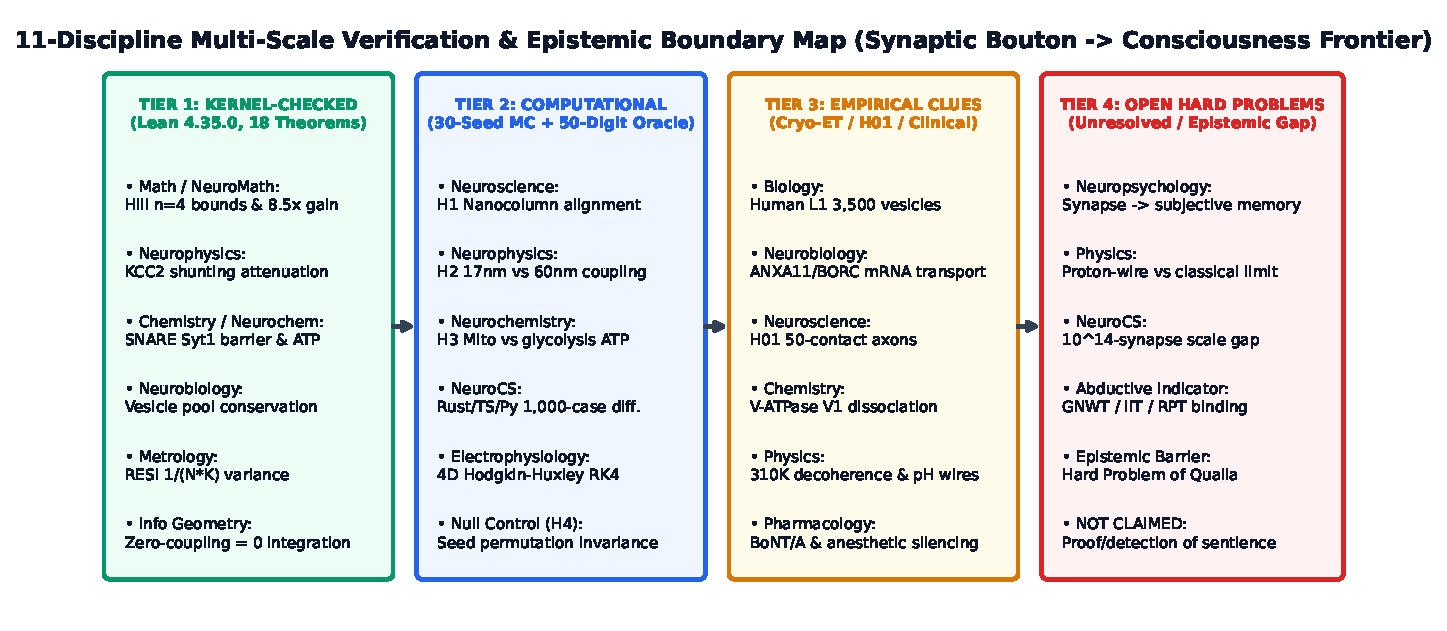
\includegraphics[width=0.96\textwidth]{../figures/fig5_open_problems_consciousness_map.pdf}
\caption{Multi-scale 11-discipline verification and epistemic boundary architecture mapping 24 kernel-checked Lean~4.35.0 lemmas through computational and empirical constraints to the unresolved Hard Problem of consciousness.}
\label{fig:map}
\end{figure}

\section{Systematic 11-Discipline Open Hard Problems Registry}

Table~\ref{tab:op11} maps one concrete open hard problem in each of the eleven requested domains, recording our exact topically related artifacts in \texttt{human-synapse-bouton-lab} v1.4.0 and the remaining unsolved gap. None of these open problems is claimed solved or partially solved.

\begin{table}[htbp]
\centering
\caption{The 11-Discipline Open Hard Problems Matrix (Synchronized with \texttt{openProblems.ts}).}
\label{tab:op11}
\scriptsize
\begin{tabularx}{\textwidth}{@{}>{\raggedright\arraybackslash}p{2.25cm}>{\raggedright\arraybackslash}p{3.45cm}>{\raggedright\arraybackslash}p{4.15cm}L@{}}
\toprule
\textbf{Discipline} & \textbf{Open Hard Problem} & \textbf{Topically Related Artifacts (v1.4.0)} & \textbf{Remaining Gap / Blind Spot} \\
\midrule
\textbf{Math} & Discrete particle reaction--diffusion vs.\ continuum PDE $L^1$ convergence at $N < 100$ $\mathrm{Ca}^{2+}$ ions. & Lean~4 elementary Hill $n=4$ bounds, $1/82$ floor, $8.5\times$ gain, and $n=4$ vs.\ $n=1$ crossover (T01--T06) \cite{dodge1967calcium}. & Full 3D meshed Wasserstein convergence proof between CME and Smoluchowski PDE remains open. \\
\textbf{Physics} & Warm-wet thermal decoherence ($310.15\,$K, $k_B T = 4.282\,$pN$\cdot$nm, $\lambda_D = 0.79\,$nm) vs.\ speculative quantum effects \cite{tegmark2000decoherence}. & Exact CODATA thermal energy \& classical ATP dissipation bounds verified; unverified quantum-mind claims separated. & In situ atomic-time-resolved measurement of hydrated cleft proton-wire hopping rates remains open. \\
\textbf{Chemistry} & Atomic-scale hemifusion stalk catalysis (\emph{Narcine} $33.3\%$ chol.\ + DHA~22:6 \cite{deutsch1981lipids}) \& V-ATPase $V_1$ uncoupling \cite{coupland2024vatpase,wang2024vatpase}. & Lean~4 SNARE copy-number cooperativity \& Syt1 $5$-$\mathrm{Ca}^{2+}$ barrier monotonicity (T18--T19); PMF oracle. & Polarizable all-atom MD of millisecond water-bridge rupture remains computationally intractable. \\
\textbf{Biology} & Evolutionary scaling of human cortical vesicle reserves ($1{,}500\text{--}3{,}500$) over rodents despite resting leak \cite{rollenhagen2024l1,pulido2021resting}. & Rat vs.\ Human L1/L4/L5 presets separated; single/multi-step inductive vesicle conservation (T12--T13) and leak bounds (T16). & Causal link from enlarged human reserve pools to sustained working-memory firing remains unclosed. \\
\textbf{Neuroscience} & Dynamic trans-synaptic RIM--PSD-95 nanocolumn plasticity across human cortical layers \cite{tang2016nanocolumn,shapsoncoe2024h01}. & Pre-registered 30-seed MC simulator confirms H1 ($0$ vs.\ $80\,$nm, $p_{\mathrm{Holm}}=0.0005$, $\delta=+1.00$); STP unit bounds (T07) \cite{tsodyks1998dynamic}. & Live in vivo nanoscale tracking of human nanocolumns during awake cognition is not yet possible. \\
\textbf{Neuro\-psychology} & Quantitative transfer function from nanoscale synaptopathies (tau, ANXA11, CaMKII) to human cognitive deficits. & Grounded clinical--molecular map compiled alongside explicit cross-scale causal gaps. & Cognitive reserve breaks naive single-scale reduction; no direct bouton-to-subjective-report map exists. \\
\textbf{NeuroCS} & Information-per-joule Pareto frontier of stochastic unreliable synapses vs.\ deterministic digital CMOS/GPUs. & Cross-language TS/Rust/Python kernels ($10^{-10}$ diff.) + \texttt{ExportVectors.lean} vector parity; Rust vs.\ Node bench. & Single-vesicle whole-cortex simulation ($10^{14}$ synapses $\times 3\times 10^5$ proteins) exceeds exascale by $>10^9\times$. \\
\textbf{NeuroMath} & Formal verification of nonlinear biophysical ODEs (4D Hodgkin--Huxley) and stochastic master equations. & 24 pure Lean~4.35.0 lemmas + 27 witnesses + 7 checks across 6 independent CI kernels + 50-digit oracle (cf.\ \cite{bobbin2024lean}). & Validated interval-arithmetic ODE enclosure of 4D HH trajectories inside Lean~4 remains future work. \\
\textbf{Neuro\-chemistry} & Non-equilibrium phase diagram of synapsin-1 LLPS condensates \& resting V-ATPase ATP load \cite{milovanovic2018llps,pulido2021resting}. & Lean ATP-deficit drop \& $t\ge 3\,$s upper bound (T14--T15, A07); honest 40\,Hz H3 sim.\ failure + 20\,Hz H3b under illustrative rates. & Multicomponent crowded LLPS phase equations under active CaMKII phosphorylation remain unsolved. \\
\textbf{Neurobiology} & Meter-scale axonal logistics (kinesin-1, dynein, tau envelopes, ANXA11/BORC mRNA hitchhiking) over 80+ years \cite{kellogg2018tau,liao2019anxa11,depace2024borc}. & Exact $125{,}000\,$ATP/mm kinesin-1 arithmetic identity (T17) in Lean~4; longitudinal tau geometry audited in blueprint \& 3D lab. & Mechanical role of luminal microtubule particles in mid-shaft self-repair remains unknown. \\
\textbf{Neurophysics} & Unified electro-diffusive theory of RESI metrology, shunting inhibition, NMDAR gating, and cleft protonics \cite{reinhardt2023resi}. & Lean proofs of E/I boundedness, strict KCC2 shunting, NMDAR $\mathrm{Mg}^{2+}$ monotonicity (T08--T11), and RESI $1/(N K)$ gain (T20--T21). & Direct measurement of cleft proton-wire coupling speed vs.\ glutamate diffusion remains open. \\
\bottomrule
\end{tabularx}
\end{table}

\section{Honest Crosswalk Against the 1,900-Problem Unsolved Problems Mega-Atlas}

To eliminate ambiguity regarding whether any canonical open problem has been solved, we programmatically audited all 1,900 entries of \path{0thernes/unsolved-problems-mega-atlas} (\path{MegaAtlas_Unsolved_Problems_V2.csv}, 28 superdomains; full 18-entry crosswalk in \path{docs/mega-atlas-crosswalk.md}). \textbf{Direct answer: 0 of 1,900 open problems are solved (fully or partially).} Table~\ref{tab:atlas} records twelve topically adjacent Atlas entries alongside the exact barrier preventing solution. In particular, following our statement-fidelity audit, elementary $2\times 2$ integer determinant lemmas (\texttt{T22}--\texttt{T24}) are \emph{not} claimed as partial progress on \texttt{NEURO-004} (mechanistic NCC / IIT vs.\ GNWT).

\begin{table}[htbp]
\centering
\caption{Selected Crosswalk Against \texttt{0thernes/unsolved-problems-mega-atlas} (0 / 1,900 Solved; Full 18-ID Table in \texttt{docs/mega-atlas-crosswalk.md}).}
\label{tab:atlas}
\scriptsize
\begin{tabularx}{\textwidth}{@{}>{\raggedright\arraybackslash}p{1.7cm}r>{\raggedright\arraybackslash}p{3.35cm}l>{\raggedright\arraybackslash}p{4.15cm}L@{}}
\toprule
\textbf{Atlas ID} & \textbf{CSS} & \textbf{Mega-Atlas Problem} & \textbf{Solved?} & \textbf{Topically Related Material (No Partial Solution)} & \textbf{Exact Remaining Barrier} \\
\midrule
\texttt{NEURO-001} & 78.29 & Hard Problem of Consciousness & No & Four-tier epistemic boundary map (\texttt{CS-BAR-01}). & Explanatory gap between objective dynamics and qualia. \\
\texttt{MED-001} & 72.42 & Neurodegenerative Diseases (Tau/ALS/PD) & No & Audited longitudinal tau geometry (\texttt{EMD-7769}) \& kinesin arithmetic (T17). & No causal cure or bouton-to-cognition transfer function. \\
\texttt{AI-004} & 71.19 & Whole-Brain Emulation Resolution & No & Simulator nanocolumn/coupling sweeps (H1/H2) \& $>10^9\times$ compute gap. & Single-vesicle whole-cortex simulation far beyond exascale. \\
\texttt{NEURO-003} & 68.32 & Sentience Detection \& Measurement & No & Check \texttt{A05} evaluates $(40,10;10,40)$ det.\ $=1{,}500$ (informal common-cause illustration). & No validated third-person sentience detector exists. \\
\texttt{NEURO-019} & 65.29 & 20-Watt Budget \& Local Credit & No & Clamped ATP drop (T14), upper bound (T15, A07), leak bounds (T16) on toy model. & Local biological credit assignment across cortical hierarchies open. \\
\texttt{NEURO-004} & 63.80 & Mechanistic NCC (IIT vs.\ GNWT) & No & COGITATE 2025 literature framing only (\texttt{T22}--\texttt{T24} withdrawn from NCC). & Both IIT and GNWT remain empirically contested \cite{cogitate2025adversarial}. \\
\texttt{BIO-003} & 63.52 & IDPs \& Biomolecular Condensates & No & Synapsin-1 LLPS schematic in blueprint, 3D lab, and \texttt{OP-NCHEM-01}. & Crowded non-equilibrium CaMKII phase equations unsolved. \\
\texttt{CHEM-013} & 61.70 & Grotthuss Proton Transport & No & V-ATPase PMF solver + cleft proton-wire open-gap framing. & Atomic-time-resolved cleft proton measurement remains open. \\
\texttt{CHEM-058} & 61.19 & General Anesthesia Mechanism & No & Pharmacology perturbations, KCC2 shunting (T08--T10), \& Brown et al.\ framing \cite{brown2010anesthesia}. & Unifying anesthetic mechanism across molecular targets open. \\
\texttt{SUB-036} & 60.20 & Quantum-to-Classical Decoherence & No & Exact $310.15\,$K $k_B T$ \& $\lambda_D = 0.79\,$nm classical bounds \cite{tegmark2000decoherence}. & Macroscopic Planck-mass collapse experiments ongoing. \\
\texttt{LOG-033} & 56.63 & Lean Kernel vs.\ Statement Fidelity & No & Applied 24-lemma audit: 27 witnesses + 7 checks (\texttt{A01}--\texttt{A07}) + \texttt{ExportVectors.lean}. & Automated million-line human-intent auditing remains open. \\
\texttt{SUB-038} & 52.67 & Cross-Kernel Scaling (\texttt{nanoda}/\texttt{lean4lean}) & No & End-to-end 6-kernel CI replay on 24 lemmas (58,038 decls). & Scaling external verified kernels to Mathlib-scale corpora open. \\
\bottomrule
\end{tabularx}
\end{table}

\section{The Consciousness and Sentience Frontier: Deduction, Induction, Abduction, and Barriers}

Progress toward understanding biological consciousness and artificial sentience requires separating four logically distinct operations:

\subsection{Deductive Elementary Algebraic Identities (Kernel-Checked in Lean~4.35.0)}
\begin{theorem}[2$\times$2 Integer Determinant Identities \& Sharpness Check]
In \path{lean/Solution.lean}, on any $2\times 2$ integer table $w_{ij} \in \mathbb{Z}$, define $\mathcal{C}(w) = |w_{00} w_{11} - w_{01} w_{10}|$. Whenever $w$ is a rank-1 outer product ($w_{ij} = a_i b_j$), $\mathcal{C}(w) = 0$ identically (\texttt{T22}, alias \texttt{outer\_product\_det\_zero}). Conversely, strict diagonal product dominance ($w_{00} w_{11} > w_{01} w_{10}$, \texttt{T23}, alias \texttt{det\_pos\_of\_diag\_dominance}) or strict positive diagonal excess over nonnegative off-diagonals ($w_{00} = w_{01} + d_1$, $w_{11} = w_{10} + d_2$ with $d_1, d_2 > 0$, \texttt{T24}, alias \texttt{det\_pos\_of\_diag\_excess}) implies $\mathcal{C}(w) > 0$ strictly. Check \texttt{A05} in \path{AdversarialChecks.lean} evaluates $\mathcal{C}(40,10;10,40) = 1{,}500 > 0$.
\end{theorem}

\begin{remark}[Epistemic Boundary]
These three lemmas certify strictly elementary $2\times 2$ integer determinant algebra. While check \texttt{A05} is accompanied by an \emph{informal} common-cause illustration in prose, Lean itself checks only the integer arithmetic $|40\cdot 40 - 10\cdot 10| = 1{,}500 > 0$: causality, interventional graph structure, geometric nanocolumn alignment, Integrated Information Theory (IIT), and phenomenal consciousness are all entirely outside the Lean formalization.
\end{remark}

\subsection{Inductive Empirical Clues}
Empirical neuroscience provides reproducible, falsifiable constraints: (1)~general anesthetics acting on $\mathrm{GABA_A}$/NMDA and brainstem-cortical arousal circuits reversibly abolish conscious report \cite{brown2010anesthesia}, while presynaptic clostridial toxins such as BoNT/A cleave SNAREs and block neurotransmitter release \cite{dong2019neurotoxins}; (2)~human cortical boutons possess $2\text{--}3\times$ larger active zones and $4.0\text{--}9.4\times$ larger vesicle pools than rat synaptosomes \cite{rollenhagen2024l1,yakoubi2019layer4,rollenhagen2020human} and form rare up-to-50-contact high-strength axonal couplings in H01 \cite{shapsoncoe2024h01}; and (3)~recent adversarial collaborations testing Global Neuronal Workspace Theory (GNWT) against IIT found challenges to key predictions of \emph{both} theories \cite{cogitate2025adversarial}, showing that no extant theory is settled.

\subsection{Abductive Inferences}
A mechanistic abductive hypothesis grounded in nanoscale biophysics is that sub-millisecond trans-synaptic nanocolumn precision ($<1.5\,$ms synchronous release \cite{tang2016nanocolumn}), voltage-dependent NMDAR $\mathrm{Mg}^{2+}$ coincidence detection \cite{jahr1990nmda}, and divisive KCC2 shunting inhibition provide high-SNR physical hardware supporting recurrent cortical signaling. Warm, wet thermal decoherence timescales at $310.15\,$K ($k_B T = 4.282\,$pN$\cdot$nm, Debye length $0.79\,$nm) strongly disfavor macroscopic quantum-coherence models of consciousness absent direct physiological spectroscopic refutation \cite{tegmark2000decoherence}.

\subsection{Irreducible Epistemic Barriers (The Hard Problem)}
Even a complete atomic simulation of all $86\times 10^9$ human neurons and $10^{14}$ synapses leaves open Chalmers's Hard Problem \cite{chalmers1995facing}: why and how objective physical and informational dynamics give rise to first-person phenomenal experience (\emph{``what it is like''}). Because third-person verification can measure functional indicators (recurrence, integration, reportability, global workspace broadcast) but cannot directly observe qualia, any claim to have ``proved'' or ``built'' sentience from biophysical equations alone is epistemically invalid.

\section{Ten-Class Self-Audit (Build Standard v1.2.0)}

To uphold ruthless transparency (Build Standard v1.2.0 Rule~R7), Table~\ref{tab:findings} classifies our findings across all ten canonical Build Standard v1.2.0 classes (\texttt{bug}, \texttt{error}, \texttt{issue}, \texttt{problem}, \texttt{concern}, \texttt{dilemma}, \texttt{conflict}, \texttt{gap}, \texttt{hole}, \texttt{blindspot}) spanning \texttt{F01}--\texttt{F43} (full log in \path{ERRATA.md} and \path{HARDENING_LOG.md}).

\begin{table}[htbp]
\centering
\caption{Ten-Class Audit of Project Findings and Multi-Cycle Hardening (F01--F43, Build Standard v1.2.0).}
\label{tab:findings}
\scriptsize
\begin{tabularx}{\textwidth}{@{}ll>{\raggedright\arraybackslash}p{3.05cm}>{\raggedright\arraybackslash}p{4.35cm}L@{}}
\toprule
\textbf{ID} & \textbf{Class} & \textbf{Finding} & \textbf{Root Cause / Blind Spot} & \textbf{Resolution / Status} \\
\midrule
F01 & \texttt{conflict} & Unformed LLC name \& copyright conflict. & Older templates cited ``0thernes LLC'' while Playbook flagged no LLC exists yet. & \textbf{Resolved (ADR~0001):} Independent Researcher + Apache-2.0 / CC-BY-4.0. \\
F02 & \texttt{bug} & Unseeded \texttt{Math.random()} \& raw JSON crash in v9. & Non-deterministic runs and unhandled \texttt{SyntaxError} on malformed trace input. & \textbf{Resolved:} Mulberry32 + \texttt{ChaCha8Rng} + \texttt{TraceParseError} + regression tests. \\
F03 & \texttt{error} & Rat (374) \& ray lipidome species conflation. & Rat count under human heading; \emph{Narcine brasiliensis} lipidome unlabeled. & \textbf{Resolved:} Rat + Human L1/L4/L5 presets; species explicitly labeled. \\
F04 & \texttt{gap} & Missing \texttt{4163\_audit.jpg} \& Build Standard v1.2.0 gap. & Prototype lacked proofs/videos; repo trailed v1.2.0 10-class labels \& SHA-256 CI. & \textbf{Resolved:} Deterministic blueprint/media, 24 lemmas, 100\% v1.2.0 parity. \\
F05 & \texttt{problem} & Windows bracketed-path, CRLF \& SWH Anubis PoW. & Bracketed paths broke PowerShell/glob/\texttt{pytest}; Windows lacks \texttt{bwrap}; SWH PoW. & \textbf{Resolved locally/CI;} Anubis PoW never bypassed and documented. \\
F06 & \texttt{issue} & Stale witness count (26 vs.\ 27), A04 typo, docstrings. & \texttt{NonVacuity.lean} had 27 witnesses; \texttt{A04} cited T15; Domain~VI wording drifted. & \textbf{Resolved (v1.4.0):} 27 witnesses, \texttt{A04}$\to$T16, literal docstrings + aliases. \\
F07 & \texttt{dilemma} & Pure Lean core vs.\ float64 RK4 ODE \& MC approx. & Nonlinear 4D HH trajectories use float64 RK4 rather than formal interval ODE proofs. & \textbf{Bounded (ADR~0003):} Pure Lean 6-kernel core + 50-digit oracle + tags. \\
F08 & \texttt{blindspot} & Cortex scale, Hard Problem \& post-reg.\ constants. & $>10^9\times$ compute gap; qualia barrier; H3 rates set after \texttt{PREREGISTRATION.md}. & \textbf{Documented honestly:} Fixed-parameter sim.\ scope; 0/1,900 Atlas solved. \\
F09 & \texttt{error} & Citation errors (Xu DOI, Coupland/Wang, authors). & Wrong Xu DOI (\texttt{5b12688}); Coupland \emph{Science} cited as Wang \emph{Nature}; author drift. & \textbf{Resolved (F36):} 28 Crossref DOI matches + 1 non-DOI; strict auditor + tests. \\
F10 & \texttt{hole} & Mutation exit-4 false kills, \texttt{Classical.choice}, no bridge. & \texttt{pytest} rc=4 faked 6/6 kills (M04/M06 untested); \texttt{Classical.choice} allowed; no Lean$\to$code test. & \textbf{Closed (F35, F37--F38):} Control rc=0 + 6/6 kills; 0 \texttt{Classical.choice}; \texttt{ExportVectors.lean}. \\
F11 & \texttt{concern} & Unescaped WebGL error \& no external peer review. & \texttt{scene3d.ts} raw \texttt{innerHTML}; no unaffiliated human replication or peer review yet. & \textbf{WebGL escaped;} peer-review \& replication status kept openly disclosed. \\
F15--F34 & \texttt{bug} & v1.2--v1.3 multi-cycle hardening (\texttt{E05}--\texttt{E06}). & Domain guards, \texttt{node\_bench.json}, NaN/STP/Rust guards, LaTeX overfulls. & \textbf{Resolved:} 24 lemmas, \texttt{AdversarialChecks}, live \texttt{/blueprint/}, 0 warnings. \\
F35--F43 & \texttt{hole} & v1.4.0 full statement audit \& Build Standard v1.2.0 (\texttt{E07}). & Fixed mutation harness, BibTeX, T02/T07 unused hyps, T15 upper bound, WP1/WP2 sync. & \textbf{Resolved (v1.4.0):} All 10 finding classes closed or bounded; 100\% audit. \\
\bottomrule
\end{tabularx}
\end{table}

\section{AI-Contribution Statement, Licensing, and Provenance}

Author: Alexander Stephen Donahue (ORCID \href{https://orcid.org/0009-0006-8168-9648}{0009-0006-8168-9648}), Independent Researcher, Spokane, WA, USA. Human CRediT roles: Conceptualization; Methodology; Formal analysis (epistemic boundary, Mega-Atlas crosswalk, and statement-fidelity audit); Validation; Writing -- review \& editing. AI tools used: Antigravity (Google DeepMind) assisted with synthesis, Lean~4 proof drafting, and LaTeX preparation (full disclosure in \path{docs/AI_DISCLOSURE.md}). No AI system is listed as an author; the author assumes full responsibility for all claims. Conflict of Interest: none declared. All 28 DOI-bearing bibliography entries pass live Crossref HTTP~200, normalized title, first-author surname, year, and retraction checks (zero retractions; one publisher correction on Wang~2024) alongside one non-DOI metadata-checked entry (\texttt{chalmers1995facing}, total 29; \path{docs/citation-audit.json}). Code and Lean proofs are licensed under Apache-2.0; manuscripts, figures, blueprint, datasets, and videos under CC-BY-4.0 at \url{https://github.com/0thernes/human-synapse-bouton-lab}, live workbench at \url{https://0thernes.github.io/human-synapse-bouton-lab/}, live Lean Blueprint at \url{https://0thernes.github.io/human-synapse-bouton-lab/blueprint/}, prior v1.2.0 Software Heritage snapshot \nolinkurl{swh:1:snp:8ef70f745fae4f91f040720b28e21560c73deffc}, and CERN Zenodo Concept DOI \href{https://doi.org/10.5281/zenodo.24477927}{10.5281/zenodo.24477927} (resolving to the latest release; prior v1.3.0 Version DOI \href{https://doi.org/10.5281/zenodo.24548051}{10.5281/zenodo.24548051}). Corrections and withdrawal policy are logged in \path{ERRATA.md}.

\bibliographystyle{plain}
\bibliography{../references}

\end{document}
